\chapter{Casos de éxito y uso real del producto}

El módulo \textit{Meta-DYNAsystem} se pensó para ser desarrollado en un plazo de tres meses, uno de aprendizaje y dos de producción real de código e implementación del proyecto.\\

Sin embargo, el tiempo de desarrollo de la aplicación embebida, desarrollada por otro lado por otra parte del equipo, llevó más tiempo. Para entonces, la distribución propia basada en \textit{GNU/Linux} ya estaba terminada.\\

El producto pudo ser \textbf{lanzado al mercado y comercializado a nivel global}, siendo adquirido por clientes que llevaban tiempo siguiendo de cerca el proyecto a la espera del lanzamiento. Esto quiere decir que tanto el dispositivo al completo como su sistema operativo dedicado intrínseco se están utilizando a día de hoy en un ambiente de producción de uso diario.\\

Pasemos a hablar sobre los \textbf{primeros compradores}. Se trata del \textbf{equipo de investigación de \textit{Ciencias del Deporte} de la \textit{Universidad Católica de la Santísima Concepción}} \textit{(Chile)}.\\

Estos usuarios ya disponen de su dispositivo enviado e instalado en sus centros de investigación, utilizando el sistema a diario para extraer datos en tiempo real del entrenamiento de sus deportistas. Veamos un par de imágenes:

\begin{figure}[H]
	\centering
	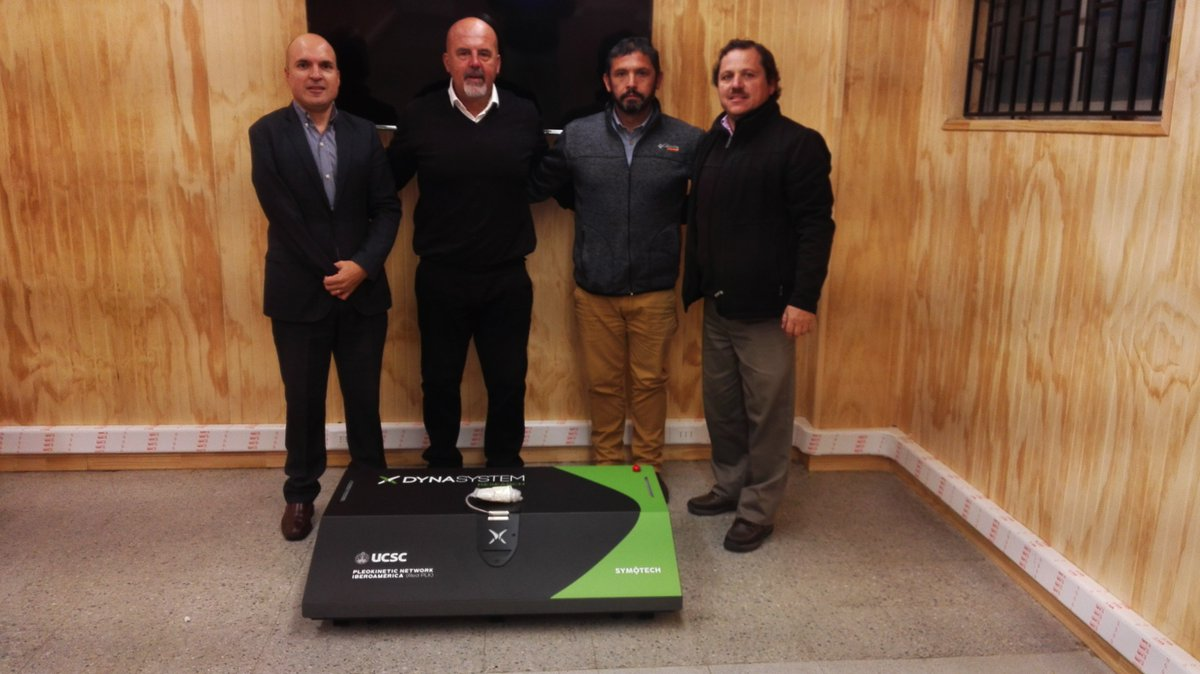
\includegraphics[width=0.9\linewidth]{imagenes/dynasystem-ucsc.jpg}
	\caption{Máquina \textit{DYNAsystem} adquirida por el equipo de investigación de Ciencias del Deporte de la \textit{UCSC (Chile)} - \textit{Twitter} oficial del producto \cite{dynasystem-ucsc}}
	\label{dynasystem-ucsc}
\end{figure}

\begin{figure}[H]
	\centering
	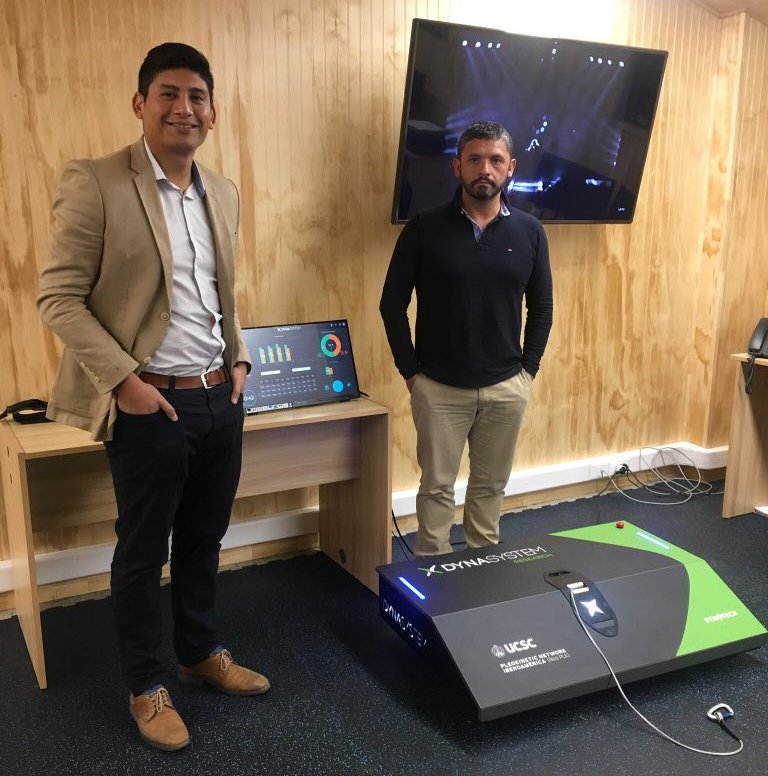
\includegraphics[width=0.7\linewidth]{imagenes/dynasystem-ucsc-2.jpg}
	\caption{Máquina \textit{DYNAsystem} adquirida por el equipo de investigación de Ciencias del Deporte de la \textit{UCSC (Chile)} - \textit{Twitter} oficial del producto \cite{dynasystem-ucsc-2}}
	\label{dynasystem-ucsc-2}
\end{figure}

Por otro lado, durante las primeras semanas de uso del dispositivo en Chile, en el equipo de desarrollo de \textit{Symotech} se siguieron implementando mejoras y avances en las capacidades del dispositivo, además de solucionar algunos errores conocidos de no demasiada importancia.\\

Gracias al sistema de actualizaciones integrado con la distribución interna al dispositivo, \textbf{se pudieron desplegar dos actualizaciones exitosas de forma remota}; actualizando tanto el software intrínseco a la electrónica como la aplicación embebida con que interacciona el usuario.\\

Veamos una captura de pantalla de la plataforma web de \textit{Hosted Mender}, servicio ya comentado previamente, donde se aprecia el éxito de la actualización finalizada.\\

En ella se muestra parte del ID del dispositivo, su tipo (basado en \textit{Raspberry Pi 3}), la versión actualmente instalada y las fechas de inicio y finalización del despliegue:

\begin{figure}[H]
	\centering
	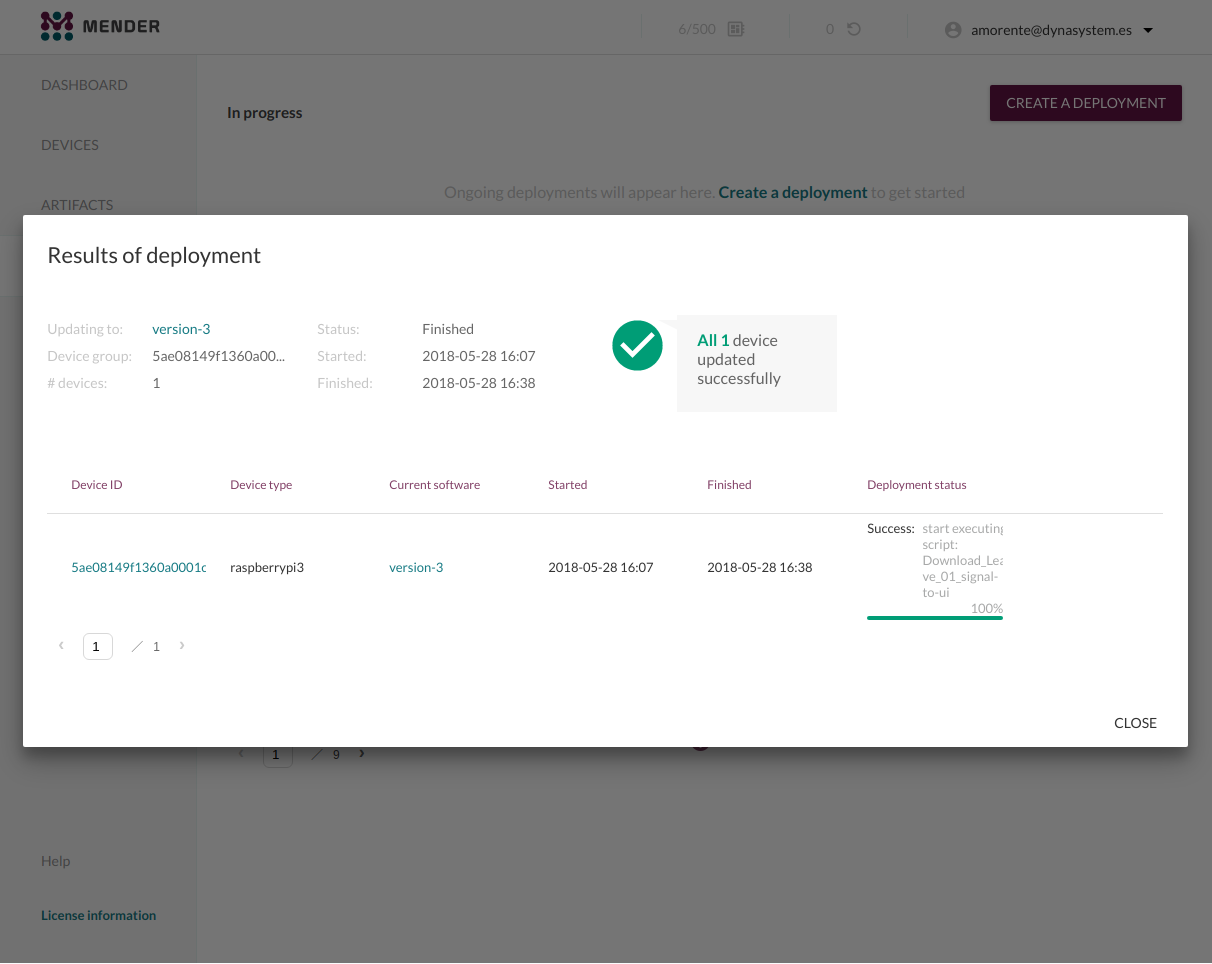
\includegraphics[width=\linewidth]{imagenes/ejemplo-actualizacion-exitosa.png}
	\caption{Muestra de la segunda actualización exitosa a la máquina instalada en la \textit{UCSC} de Chile - Adrián Morente Gabaldón \textit{[plataforma web de Hosted Mender]}}
	\label{dynasystem-ucsc-mender}
\end{figure}

\noindent\makebox[\linewidth]{\rule{\textwidth}{0.4pt}}\\

Actualmente, a mediados de junio de 2018, se han producido más ventas e instalaciones del dispositivo a nivel nacional con actualizaciones realizadas, pero no disponemos de medios de carácter multimedia que lo prueben (como imágenes o vídeos).\\

Sin embargo, en la ya mencionada cuenta de \textit{Twitter} oficial del producto se pueden encontrar muchos medios de publicidad y difusión del dispositivo, con gente ajena al proyecto (fisioterapeutas y deportistas de todo tipo) probándolo a diario y dando su visto bueno: \href{https:www.twitter.com/dynasystem\_}{enlace a \textit{Twitter}} \cite{twitter-dynasystem}.

\newpage